%% document class file for the preparation of a paper
%% for the International Conference ICCAS 2020
%% global option 'fleqn' ensures equations flush left.
%% set '10pt' and 'twocolumn' options.
\documentclass[10pt,twocolumn]{ICCAS}
\usepackage[a4paper, left=20mm, right=20mm, top=25mm, bottom=25mm]{geometry}
\usepackage{amsmath, amssymb}
\usepackage{bm}

%--- Custom Commands ---
\newcommand{\tr}{\operatorname{tr}}
\newcommand{\ud}{\,\mathrm{d}}
\newcommand{\R}{\mathbb{R}}
\newcommand{\xtilde}{\tilde{\bm{x}}}
\newcommand{\xhat}{\hat{\bm{x}}}
\newcommand{\xbar}{\bar{\bm{x}}}
\newcommand{\xhatbar}{\hat{\bar{\bm{x}}}}
\newcommand{\Wtilde}{\tilde{\mathbf{W}}}
\newcommand{\What}{\hat{\mathbf{W}}}
\newcommand{\W}{\mathbf{W}}
\newcommand{\Vtilde}{\tilde{\mathbf{V}}}
\newcommand{\Vhat}{\hat{\mathbf{V}}}
\newcommand{\Vstar}{\mathbf{V}^*}
\newcommand{\diag}{\operatorname{diag}}
\newcommand{\Lambdamat}{\mathbf{\Lambda}}

\newtheorem{assumption}{Assumption}

%%%%%%% set heading and page number hear %%%%%%%%%%
% % Do not put page numbers for submission.
%\setcounter{page}{101}

\usepackage{xcolor}
\usepackage{kotex}

% 
\newcommand{\KHCH}[1]{{\color{RoyalPurple} [KH: #1]}} % Kyunghwan's
\newcommand{\MSRY}[1]{{\color{Peach} [MS: #1]}} % Myeongseok's 
\newcommand{\SHJH}[1]{{\color{green} [SH: #1]}} % Seunghun's 
\newcommand{\DHHO}[1]{{\color{magenta} [DH: #1]}} % Donghwa's 

\newcommand{\etal}{\textit{et~al.\ }}
\newcommand\eg{\textrm{e.g.,\ }}
\newcommand\ie{\textrm{i.e.,\ }}

\newcommand{\colorLine}[2]{[\tikz[baseline=(current bounding box.base)]{\draw[color=#1,
#2,line width=2pt] (0,3pt) -- (1.5em,3pt);}]}

\newcommand{\DHHO}[1]{\textcolor{magenta}{#1}}
\newcommand{\KHCO}[1]{\textcolor{red}{#1}}


\begin{document}

\title{Integral Error-Based Adaptive Neural Identifier for a Class of Uncertain Nonlinear Systems}

\author{Donghwa Hong${}^{1}$ and Kyunghwan Choi${}^{2*}$ }

\affils{ ${}^{1}$Department of Mechanical Robotics Engineering, GIST, \\
Seoul, 13391, Korea (first@hankook.ac.kr) \\
${}^{2}$Department of Mechanical Engineering, Cho, \\
Seoul, 13391, Korea (second@hankook.ac.kr) {\small${}^{*}$ Corresponding author}}

%\thanks{ \noindent
%   This paper is supported by my funding agencies.
%  }
\abstract{
This paper presents a robust online neural network (NN) identifier for uncertain nonlinear systems, focusing on online system identification and function approximation. The proposed method employs a cumulative error cost function with a forgetting factor to enable real-time learning of unknown nonlinear dynamics. A rigorous Lyapunov-based stability analysis guarantees Uniform Ultimate Boundedness (UUB) of the identification error. Comparative analysis with state error-based gradient descent methods highlights the improved stability and convergence properties of the proposed approach. The results demonstrate that the method enables effective online identification and function approximation for a wide range of nonlinear systems.
}


\keywords{
Online System Identification, Neural Networks, Adaptive Control, Stability Analysis, Nonlinear Dynamics
}

\maketitle

%-----------------------------------------------------------------------
\section{Introduction}
System identification is the process of estimating the dynamic model of an unknown plant from input-output data, which is essential for controller design and state estimation. In particular, when the system dynamics are nonlinear or time-varying, the importance of online identification becomes more pronounced. Offline identification techniques assume large batches of data and lack real-time adaptability, making them unsuitable for dynamic environments. In contrast, online identification updates the model in real time, enabling the tracking of changing system characteristics, and is thus indispensable in dynamic control applications.

Traditional online system identification methods mainly employ Recursive Least Squares (RLS)-based algorithms. RLS updates parameters by weighting past data and guarantees convergence when the system is static. However, the forgetting factor used in RLS presents a trade-off between convergence speed and tracking ability, and the choice of an appropriate forgetting factor greatly affects real-time estimation performance. To address this issue, variable forgetting factor (VFF) techniques have been proposed, which adaptively adjust the forgetting factor.

Neural network-based identification methods have been actively studied due to their flexible modeling capabilities for nonlinear systems. Neural networks possess universal approximation properties, meaning that with appropriate size, structure, and weights, they can approximate any continuous nonlinear function arbitrarily well over a compact set, thus effectively learning complex nonlinearities. For example, multilayer perceptrons or recurrent neural networks can be used as identification models to learn input-output relationships. 
The conventional backpropagation algorithm updates neural network weights by minimizing an instantaneous squared error cost function, but this approach inherently focuses only on instantaneous errors, making it difficult to guarantee long-term parameter convergence. To enhance robustness, stabilization techniques such as $\sigma$-modification and composite adaptation have been proposed.

The limitations of existing methods are as follows. First, most algorithms use cost functions that minimize instantaneous errors, causing model parameters to focus only on momentary discrepancies and making it difficult to achieve accurate function approximation over the entire time interval. Second, persistent excitation (PE) conditions are often required for parameter convergence in neural network identification, but PE may be lost once the control objective is achieved and the system reaches steady state. Third, in nonlinear system identification and control, stability proofs are often lacking, making practical application to real systems difficult.

This paper proposes a robust online neural network identification method that applies a cumulative error cost function with a forgetting factor to overcome the limitations of previous studies. Specifically, by defining a new cost function that accumulates identification errors at all time points, the method aims to minimize the overall error in a balanced manner. In addition, a variable forgetting factor is introduced to maintain adaptability to recent data while gradually reducing the influence of past information. The proposed method is rigorously analyzed using Lyapunov-based stability analysis to guarantee the Uniform Ultimate Boundedness (UUB) of the identification error. Comparative analysis with state error-based gradient descent methods demonstrates the improved stability and convergence properties of the proposed approach. The results of this study show that the method enables effective online identification and function approximation for a wide range of nonlinear systems.
%-----------------------------------------------------------------------
\section{Problem Formulation}
\subsection{Model Dynamics}

Consider the nonlinear system
\begin{equation}
    \dot{\bm{x}}(t) = \underbrace{\bm{f}(\bm{x}, \bm{u})}_{known} + \underbrace{\bm{h}(\bm{x}, \bm{u})}_{unknown}
    \label{eq:realsystem}
\end{equation}

where $\bm{x} \in \mathbb{R}^n$ is the state vector and $\bm{u} \in \mathbb{R}^m$ is the control input vector, and $\bm{f}(\cdot)$ represents the known part of the system dynamics, and $\bm{h}(\cdot)$ denotes the unknown nonlinear dynamics or disturbances.
\subsection{Neural Network Identifier}
To design a identifier, some assumptions are needed as follows : 
\begin{assumption}
The ideal weights $\mathbf{W}, \mathbf{V}$ are bounded. The disturbance $w(t)$ is bounded by $\|w(t)\| \le w_M$. The activation function $\sigma$ and its derivatives are bounded.\\
\end{assumption}

\begin{assumption}[Open-Loop Stability]
The open-loop system \eqref{eq:realsystem} is stable, which implies that the state vector $\bm{x}(t)$ is bounded in $L_\infty$.\\ 
\end{assumption}
By adding and subtracting ${\bf{A}}\bm{x}$ from . So, the system is described by:
\begin{equation}
    \dot{\bm{x}}(t) = \bf{A}\bm{x}(t) + \bm{g}(\bm{x}, \bm{u}) + \bm{h}(\bm{x}, \bm{u})
    \label{eq:system}
\end{equation}
where $\mathbf{A} \in \R^{n \times n}$ is an arbitrary Hurwitz matrix, $\bm{g}(\bm{x},\bm{u}) = \bm{f}(\bm{x}, \bm{u}) - {\mathbf{A}} \bm{x} $, which is the known nonlinear function.

Then, the identifier model can be selected as:
\begin{equation}
    \dot{\xhat}(t) = {\mathbf{A}}\bm{\xhat}(t) + \bm{g}(\bm{x}, \bm{u}) + \bm{\hat{h}}(\xhatbar)
    \label{eq:identifier}
\end{equation}
where the NN output is $\bm{\hat{h}}(\bm{\hat{x}},\bm{u}) = \What^T \sigma(\Vhat^T \xhatbar)$. Here, $\What \in \R^{h \times n}$ and $\Vhat \in \R^{d \times h}$ are the estimated weight matrices. The NN input $\xhatbar$ is constructed from the estimated states $\xhat$ and $\bm{u}$.
Defining the errors $\xtilde = \bm{x} - \xhat$, $\Wtilde = \bf{W} - \What$, and $\Vtilde = \bf{V} - \Vhat$, the error dynamics are given by:
\begin{equation}
    \dot{\xtilde} = {\mathbf{A}}\bm{\xtilde} + {\Wtilde}^{T} \sigma(\Vhat^T \bm{\xhatbar}) + w(t)
    \label{eq:error_dyn_final}
\end{equation}
where $w(t) = {\mathbf{W}}^T\left(\sigma({\mathbf{V}}^T\bm{\xbar}) - \sigma(\Vhat^T\xhatbar)\right) + \epsilon(x)$ is the lumped disturbance term.








\section{Proposed Method}

\subsection{Integral Adaptive Law based Gradient Descent}
A common approach to update the weights of a neural network is to minimize the cost function defined as the squared error. Consider the plant model \eqref{eq:system} and the identifier model \eqref{eq:identifier}. Given Assumption 2, if the weights of the NLPNN are updated according to
\begin{align}
    \dot{\mathbf{\What}} &= -\eta_1\left(\frac{\partial J}{\partial \hat{\mathbf{W}}}\right) - \rho_1\|\tilde{\bm{x}}\|\hat{\mathbf{W}},\\
    \dot{\mathbf{\Vhat}} &= -\eta_2\left(\frac{\partial J}{\partial \hat{\mathbf{V}}}\right) - \rho_2\|\tilde{\bm{x}}\|\hat{\mathbf{V}},
\end{align}
where $\eta > 0$ is the learning rate, and $\rho > 0$ is the leakage term.

And the cost function is defined as
\begin{equation}
J = \frac{1}{2} \int_{0}^{t} e^{-\lambda(t-\tau)} {\xtilde(\tau)}^T \xtilde(\tau) \ud\tau 
\end{equation} 
where $\lambda > 0$ is called forgetting factor. This function accumulates the squared error over time, with a forgetting factor that gradually reduces the influence of past errors.

Since the cost functional is of an integral form, we first introduce the filtered error signal $\bm{z}(t)$ to construct the update laws.
\begin{equation}
    \bm{z}(t) = \int_{0}^{t} e^{-\lambda(t-\tau)} \xtilde(\tau) \ud\tau
    \label{eq:filter_z}
\end{equation}
\begin{equation}
    \dot{\bm{z}} = - \lambda\bm{z} + \xtilde
    \label{eq:filter_z_dot}
\end{equation}
Let us define
\begin{align*}
    \text{net}_{\hat{\mathbf{V}}} &= \hat{\mathbf{V}}\hat{\bm{x}}  \\
    \text{net}_{\hat{\mathbf{W}}} &= \hat{\mathbf{W}}\sigma(\hat{\mathbf{V}}\hat{\bm{x}}).
\end{align*}
Therefore, by using the chain rule $\frac{\partial J}{\partial \hat{\mathbf{W}}}$ and $\frac{\partial J}{\partial \hat{\mathbf{V}}}$ can be computed according to
\begin{align*}
    \frac{\partial J}{\partial \hat{\mathbf{W}}} &= \frac{\partial J}{\partial \text{net}_{\hat{\mathbf{W}}}} \cdot \frac{\partial \text{net}_{\hat{\mathbf{W}}}}{\partial \hat{\mathbf{W}}} \\
    \frac{\partial J}{\partial \hat{\mathbf{V}}} &= \frac{\partial J}{\partial \text{net}_{\hat{\mathbf{V}}}} \cdot \frac{\partial \text{net}_{\hat{\mathbf{V}}}}{\partial \hat{\mathbf{V}}},
\end{align*}
where
\begin{align*}
    \frac{\partial J}{\partial \text{net}_{\hat{\mathbf{W}}}} 
    &= \frac{\partial J}{\partial \tilde{\bm{x}}} \frac{\partial \tilde{\bm{z}}}{\partial \hat{\bm{x}}} \frac{\partial \hat{\bm{x}}}{\partial \text{net}_{\hat{\mathbf{W}}}} = -{\bm{z}}^T \frac{\partial \hat{\bm{x}}}{\partial \text{net}_{\hat{\mathbf{W}}}}, \nonumber \\
    \frac{\partial J}{\partial \text{net}_{\hat{\mathbf{V}}}} 
    &= \frac{\partial J}{\partial \tilde{\bm{x}}} \frac{\partial \tilde{\bm{x}}}{\partial \hat{\bm{x}}} \frac{\partial \hat{\bm{x}}}{\partial \text{net}_{\hat{\mathbf{V}}}} = -{\bm{z}}^T \frac{\partial \hat{\bm{x}}}{\partial \text{net}_{\hat{\mathbf{V}}}}
\end{align*}
and
\begin{align*}
    \frac{\partial \text{net}_{\hat{\mathbf{W}}}}{\partial \hat{\mathbf{W}}} &= \sigma(\hat{\mathbf{V}}\hat{\bm{x}}) \nonumber \\
    \frac{\partial \text{net}_{\hat{\mathbf{V}}}}{\partial \hat{\mathbf{V}}} &= \hat{\bm{x}}.
\end{align*}
We modify the original BP algorithm such that the static approximations of $\frac{\partial \hat{\bm{x}}}{\partial \text{net}_{\hat{\mathbf{W}}}}$ and $\frac{\partial \hat{\bm{x}}}{\partial \text{net}_{\hat{\mathbf{V}}}}$ ($\dot{\hat{\bm{x}}} = 0$) can be used.
\begin{align*}
    \frac{\partial \hat{\bm{x}}}{\partial \text{net}_{\hat{\mathbf{W}}}} &\approx -\mathbf{A}^{-1} \nonumber \\
    \frac{\partial \hat{\bm{x}}}{\partial \text{net}_{\hat{\mathbf{V}}}} &\approx -\mathbf{A}^{-1}\hat{\mathbf{W}}(\mathbf{I} - \mathbf{\Lambda}(\hat{\mathbf{V}}\hat{\bm{x}})), 
\end{align*}
where
\begin{align*}
    \mathbf{\Lambda}(\hat{\mathbf{V}}\hat{\bm{x}}) = \diag\{\sigma_i^2(\hat{\mathbf{V}}_i\hat{\bm{x}})\}, \quad i=1,2,\dots,m.
\end{align*}
Then, the update laws for the weights $\What$ and $\Vhat$ can be expressed as:
\begin{align}
    \dot{\What} &= -\eta_1 \left(\bm{z}^{T} \bm{A}^{-1}  \right)^{T} \sigma(\Vhat^T\xhatbar)^T - \rho_1 \|\xtilde\| \What \label{eq:update_W_robust} \\
    \dot{\Vhat} &= -\eta_2 \xhatbar \left( \bm{z}^T \bm{A}^{-1} \What (\mathbf{I} - \mathbf{\Lambda}({\mathbf{\hat{V}}}{\bm{\hat{x}}})) \right)^T - \rho_2 \|\xtilde\| \Vhat \label{eq:update_V_robust}
\end{align}

\subsection{Stability Analysis}

To analyze the stability of the system described by \eqref{eq:error_dyn_final} with the update laws \eqref{eq:update_W_robust}-\eqref{eq:update_V_robust}, we will use Lyapunov's direct method. The goal is to show that the errors $\xtilde$, $\Wtilde$, and $\Vtilde$ are Uniformly Ultimately Bounded (UUB).
\begin{theorem}
For the system given by \eqref{eq:error_dyn_final} with the update laws \eqref{eq:update_W_robust}-\eqref{eq:update_V_robust}, all signals in the system ($\xtilde, \Wtilde, \Vtilde$) are Uniformly Ultimately Bounded.
\end{theorem}

\begin{proof}
The stability proof is conducted in two steps using a cascaded system approach.

% \textbf{Step 1: UUB Analysis of the $(\xtilde, \Wtilde)$ Subsystem}

We first prove the boundedness of the state error $\xtilde$ and the output layer weight error $\Wtilde$. This is possible because the term $\sigma_v = \sigma(\Vhat^T \xhatbar)$ in the error dynamics \eqref{eq:error_dyn_final} is always bounded, regardless of the value of $\Vhat$, due to the bounded nature of the activation function $\sigma$.

Consider the Lyapunov function candidate for the first subsystem:
\begin{align}
    L =\; & \frac{1}{2}\xtilde^T \mathbf{P}_1 \xtilde \notag + \frac{1}{2}\tr(\Wtilde^T \rho^{-1}\Wtilde) \notag \\
    & + \frac{1}{2} \int_{0}^{t} e^{-\lambda(t-\tau)} \xtilde(\tau)^T \mathbf{P}_2 \xtilde(\tau) \ud\tau
\end{align}
Its time derivative, after substituting the error dynamics, is:
\begin{align*}
    \dot{L} =\; & -\frac{1}{2}\xtilde^T(\mathbf{Q}_1 - \mathbf{P}_2)\xtilde+ \xtilde^T\mathbf{P}_1 (\Wtilde^T \sigma_v + w) \\
    &+ \tr(\dot{\Wtilde}^T\rho^{-1} \Wtilde) - \lambda L_{\text{int}}
\end{align*}
where $\sigma_v = \sigma(\Vhat^T\xhatbar)$, $\mathbf{Q} = \mathbf{Q}_1 - \mathbf{P}_2 > 0$, and $L_{\text{int}} = \frac{1}{2} \int_{0}^{t} e^{-\lambda(t-\tau)} \xtilde(\tau)^T \mathbf{P}_2 \xtilde(\tau) \ud\tau$.\\
And we substitute the update law \eqref{eq:update_W_robust} using $\dot{\Wtilde} = -\dot{\What}$. 
\begin{align*}
    \tr(\dot{\Wtilde}^T \rho^{-1}\Wtilde) 
    &= \tr\Big( \big(\eta_W \mathbf{A}^{-T}\bm{z}\sigma_v^T + \rho \|\xtilde\| \What\big)^T \rho^{-1}\Wtilde \Big) \\
    &= {\eta_W}\tr(\sigma_v \bm{z}^T l_1 \Wtilde)\\
    &+ \|\xtilde\| \tr(\What^T \Wtilde)
\end{align*}
where $l_1 = \mathbf{A}^{-1} \rho^{-1}$.
We expand the leakage term by substituting $\What =\bf{W} - \Wtilde$:
\begin{align*}
    \|\xtilde\| \tr(\What^T\Wtilde) &= \|\xtilde\| \tr((\bf{W} - \Wtilde)^T\Wtilde)\\&= -\|\xtilde\| \|\Wtilde\|^{2}+\|\xtilde\| \|\bf{W}\|\|\Wtilde\|
\end{align*}
Substituting this back into the $\dot{L}$ expression:
\begin{align*}
    \dot{L} \le &-\frac{1}{2}\xtilde^T\mathbf{Q}\xtilde  -\|\xtilde\| \|\Wtilde\|^{2} - \lambda L_{\text{int}} \\
    & + \xtilde^T\mathbf{P}_{1} (\Wtilde^T \sigma_v + w) + \eta_W \tr(\sigma_v {\bm{z}^T} l_{1} \Wtilde) \\
    &+  \|\xtilde\| \|\mathbf{W}\|\|\Wtilde\|
\end{align*}
Moreover, we have
\begin{align*}
    |\xtilde^T\mathbf{P}_1 \Wtilde^T \sigma_v| &\le \|\xtilde\|\|\mathbf{P}_1\|(\|\Wtilde\| \sigma_{M} + \bar{w})\\
    \|\xtilde\| \|\bf{W}\|\|\What\| &\le \|\xtilde\|\|\Wtilde\| W_M \\
        |\eta_W \tr(\sigma_v \bm{z}^T l_1 \Wtilde)|
    &\le \eta_W \|\sigma_v\| \|\bm{z}\| \|l_1\| \|\Wtilde\| \\
    &\le \eta_W \sigma_M \frac{\sqrt{n}}{\lambda} \|\xtilde\| \|l_1\| \|\Wtilde\|.
\end{align*}
where $\|W\|\le W_M$, $\|\sigma(\xhatbar)\|\le \sigma_M$, and
because $\bm z(t)$ is the state of the first-order filter~\eqref{eq:filter_z}
driven by $\xtilde(t)$, its 2-norm satisfies
\begin{align*}
    \|\bm z(t)\|
    &= \Bigl\| \int_{0}^{t} e^{-\lambda(t-\tau)} \xtilde(\tau)\,\mathrm d\tau \Bigr\| \notag\\
    &\le \int_{0}^{t} e^{-\lambda(t-\tau)} \|\xtilde(\tau)\|\,\mathrm d\tau \notag\\
    &\le \|\xtilde\|_{\infty} \int_{0}^{t} e^{-\lambda(t-\tau)}\,\mathrm d\tau \notag\\
    &= \frac{1-e^{-\lambda t}}{\lambda}\,\|\xtilde\|_{\infty} \notag\\
    &\le \frac{\sqrt{n}}{\lambda}\,\|\xtilde\|_{\infty} \notag\\
    &\le \frac{\sqrt{n}}{\lambda}\,\|\xtilde\| \quad (\text{since } \|\xtilde\|_{\infty}\le\|\xtilde\|).
\end{align*}
with $n$ denoting the state dimension. Then, the inequality becomes:
\begin{align*}
    \dot{L} \le 
    & -\frac{1}{2}\lambda_{\min}(\mathbf{Q})\|\xtilde\|^2 - \|\xtilde\|\|\Wtilde\|^2 - \lambda L_{\text{int}} \notag \\
    &+ \|\xtilde\|\|\mathbf{P}_1\|(\|\Wtilde\| \sigma_{M} + \bar{w}) \\
    &+ \|\xtilde\| W_M \|\Wtilde\| 
    + \eta_W \sigma_M \frac{\sqrt{n}}{\lambda}\|\xtilde\| \|l_1\| \|\Wtilde\|
    \label{eq:Ldot_ineq_full}
\end{align*}
By completing the squares for the terms involving $\|\hat{W}\|$, we look for conditions on $\|x\|$ which are independent of the neural network weights error and also make the time derivative of the Lyapunov candidate negative.
\begin{align}
    \dot{L} \le & - \|\xtilde\| \|\Wtilde\|^2 + k_b\|\xtilde\| \|\Wtilde\| \notag \\
    & - \frac{1}{2}\lambda_{\min}(\mathbf{Q})\|\xtilde\|^2 
    + \|\xtilde\|\|\mathbf{P}_1\|w_M 
    - \lambda L_{\text{int}}
\end{align}
where $k_b = \|\mathbf{P}_1\|\sigma_M + W_M + \eta_W\sigma_M \frac{\sqrt{n}}{\lambda} \|\mathbf{A}^{-1}\rho_1^{-1}\|$. The terms involving $\Wtilde$ are of the form $-(\|\xtilde\|)\|\Wtilde\|^2 + (k_b\|\xtilde\|)\|\Wtilde\|$.\\ 
By completing the square, this is bounded above by $\frac{(k_b\|\xtilde\|)^2}{4|\xtilde\|} = \frac{k_b^2}{4}\|\xtilde\|$.
The final inequality for $\dot{L}$ is:
\begin{align}
    \dot{L} \le -\frac{1}{2}\lambda_{min}(\mathbf{Q})\|\xtilde\|^2 - \lambda L_{\text{int}}+ \left( \|\mathbf{P}_1\|\bar{w} + \frac{k_b^2}{4} \right)\|\xtilde\|
\end{align}
To find a sufficient condition that guarantees $\dot{L} \le 0$ and subsequently derive the ultimate bound, we can analyze a simpler upper bound. Since the term $-\lambda L_{int}$ is always non-positive, it can be omitted from the right-hand side while the inequality still holds. The analysis thus proceeds with the remaining terms :
\begin{align}
    \|\xtilde\|\ge\frac{2\left( \|\mathbf{P}_1\|\bar{w} + k_b^2 \right)}{\lambda_{min}(\mathbf{Q})}=b
\end{align}
Furthermore, the above condition on $\|\xtilde\|$ guarantees the negative semi-definiteness of $\dot{L}$ and therefore, ultimate boundedness of $\xtilde$.
In fact, $\dot{L}$ is negative definite outside the ball with radius $b$.\\ 

\end{proof}

\subsection{parameter tuning guidelines}

The proposed method requires tuning of several parameters, including the learning rates $\eta_1$, $\eta_2$, the forgetting factor $\lambda$, and the leakage terms $\rho_1$, $\rho_2$. The following guidelines can be used for parameter selection:
\begin{itemize}
    \item \textbf{Learning Rates ($\eta_1$, $\eta_2$)}: These should be chosen small enough to ensure stability but large enough to allow for fast learning. A common practice is to start with small values (e.g., $0.01$) and adjust based on the convergence speed observed in simulations.
    \item \textbf{Forgetting Factor ($\lambda$)}: This parameter controls how much past errors influence the current cost function. A typical value is around $0.1$, but it can be adjusted based on the system dynamics and the desired responsiveness of the identifier.
    \item \textbf{Leakage Terms ($\rho_1$, $\rho_2$)}: These terms help prevent unbounded growth of the weights. They can be set to small values (e.g., $0.001$) to ensure that the weights do not diverge while still allowing for sufficient adaptation.
\end{itemize}
\noindent

\section{Simulation}

The dynamics of an $n$-degree-of-freedom robot manipulator can be described by the following nonlinear state-space model:
\begin{equation}
    \bm{M}(\bm{q})\ddot{\bm{q}} + \bm{C}(\bm{q}, \dot{\bm{q}})\dot{\bm{q}} + \bm{G}(\bm{q}) + \bm{\tau_{d}}= \bm{\tau}
    \label{eq:robot_dynamics}
\end{equation}
where $\bm{q} \in \R^{n}$ is the joint position vector, $\dot{\bm{q}}$ and $\ddot{\bm{q}}$ are the joint velocity and acceleration vectors, $\bm{M}(\bm{q}) \in \R^{n \times n}$ is the positive definite inertia matrix, $\mathbf{C}(\bm{q}, \dot{\bm{q}}) \in \R^{n \times n}$ is the Coriolis/centrifugal matrix, $\bm{G}(\bm{q}) \in \R^n$ is the gravity vector, and $\bm{\tau} \in \R^n$ is the control input.
To generalize the system for identification of an unknown nonlinear function, we consider a Hamiltonian structure where the dynamics are partitioned into known and unknown components. 
\begin{align}
    \begin{bmatrix}
        \dot{\bm{q}} \\ \dot{\bm{p}}
    \end{bmatrix}
    =
    \underbrace{
    \begin{bmatrix}
        \mathbf{0} & \mathbf{I} \\
        -\mathbf{I} & \mathbf{0}
    \end{bmatrix}
    \begin{bmatrix}
        \frac{\partial{H}}{\partial{p}} \\ \frac{\partial{H}}{\partial{q}}
    \end{bmatrix}
    +
    \begin{bmatrix}
        \mathbf{0} \\
        \mathbf{I}
    \end{bmatrix} \bm{\tau}}_{\text{known}}
    -
    \underbrace{
    \begin{bmatrix}
        \mathbf{0} \\
        \mathbf{I}
    \end{bmatrix} \bm{\tau_d}
    }_{\text{unknown}}
    \label{eq:robot_dynamics_nonlinear}
\end{align}

where $\bm{p} = \bm{M}(\bm{q})\dot{\bm{q}}$ is the generalized momentum, $\bm{x} = [\bm{q}^{T} \ \bm{p}^{T}]$ is the state vector composed of joint positions and momenta, and $H(\bm{q}, \bm{p})$ is the Hamiltonian (total energy) of the system. The first term on the right-hand side represents the intrinsic system dynamics derived from the Hamiltonian structure, while the second and third terms correspond to the control input and dissipative torque, respectively.


\subsection{Figures and tables}
All figures and tables should be placed after their first 

\newpage
\noindent
mention in the text. Large
figures and tables may span across both columns. Scanned images (e.g., line art, photos)
can be used if the output resolution is at least 600 dpi.

\begin{figure}[thb]
\begin{center}
%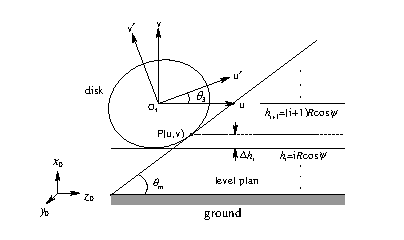
\includegraphics[height=3cm]{test.eps}
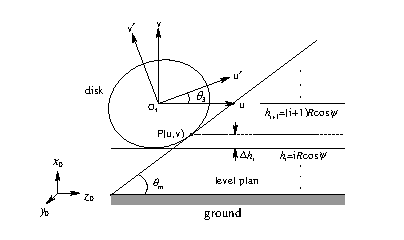
\includegraphics[width=6.5cm]{test.eps}
\caption{\label{test}The caption should be placed after the figure.}
\end{center}
\end{figure}

Figure captions should be below the figures; table captions should be above the tables.
They should be referred to in the text as, for example, Fig. \ref{test}, or Figs.
1$\sim$3.\\

\begin{table}[ht]
    \centering
    \begin{tabularx}{\linewidth}{|>{\centering\arraybackslash}X|>{\centering\arraybackslash}X|>{\centering\arraybackslash}X|>{\centering\arraybackslash}X|}
        \hline
        \diagbox[width=4.7pc, height=1.5pc]{~}{~} & A & B & C \\
        \hline
        (1) & 150\% & 16.3\% & 18.2\% \\
        \hline
    \end{tabularx}
    \caption{Your table caption here}
    \label{tab:your_label}
\end{table}

\subsection{Equations}
Equation numbers should be Arabic numerals enclosed in parentheses
on the right-hand margin. They should be cited in the text as, for
example, Eq. (1), or Eqs. (1)$\sim$(3). Equations are located in the middle and equation numbers are located at the end. Punctuate equations with commas or periods when
they are part of a sentence. For example,
\begin{align}
&\dot{x} =  Ax+Bu, \label{eq.1}\\
&y  =  Cx+Du. \label{eq.2}
\end{align}
 
\subsection{References} References should appear in a separate
bibliography at the end of the paper, with items referred to by
numerals in square brackets [1, 4-5]. Times New Roman 10pt is used
for references.
%\cite{ref1}. Times New Roman 10pt is used for references.

\section{Page Numbers}
Do not put a page number in the manuscript PDF.



%\section*{ACKNOWLEDGEMENT}
%
%This paper has been supported by NRF of Korea in 2021.


%%%%%%%%%%%%%%%%% BIBLIOGRAPHY IN THE LaTeX file !!!!! %%%%%%%%%%%%%%%%%%%%%%
%%---------------------------------------------------------------------------%%
%
\begin{thebibliography}{99}

\bibitem{ref1}
J. H. Bong, ``Controlling the parasite,'' in \textit{Proc. of International Conference on Control, Automation and Systems}, pp. 0209-0210, 2020


\bibitem{ref2}
A. Alice and B. Bob, ``Nonlinear unstable systems,'' \textit{International Journal of Control, Automation, and Systems}, vol. 23, no. 4, pp. 123–145, 1989.

\bibitem{ref3}
M. Young, \textit{The Technical Writer's Handbook}, Mill Valley, Seoul, 1989.



\end{thebibliography}
%
%%--------------------------------------------------------------------%%

\end{document}
